%Sidenote from Angie: Green text after a percentage sign includes notes to the LaTeX code, useful tips and tricks I thought you might need ⁠— feel free to read them for extra info on this template.

%~~~~~~~~~~~~~~~~~~~~~~~~~~~~~~~~~~~~~~~~~~~~~~~~~~~~~~~%
% Changelog 7.21: Lab now moving from remote learning to physical laboratory, please ignore any comments after '% OLD TEXT IGNORE:'
%Changelog 10.21: Fixed the formatting of RSC referencing style 
%Changelog 1.22: Reviewed before the start of Semester 2, fixed some wording/clarification issues
%Changelog 5.22: Reviewed after semester 2, fixed some wording/clarification issues, removed OLD TEXT
%~~~~~~~~~~~~~~~~~~~~~~~~~~~~~~~~~~~~~~~~~~~~~~~~~~~~~~~%

\documentclass[twocolumn]{article} %sets the type of the document that you compile, for just now it is an article - specifically one with a two-column formatting

%~~~~~~~ Packages ~~~~~~~~~%
% Please don't be scared by the chunk of code below, these are just some handy tools that make using LaTeX easier, you can read more on your own time, for example here: https://www.latex-tutorial.com/tutorials/packages/
%\usepackage{amsmath}
% \usepackage{caption}
% \usepackage{subcaption}
\usepackage[utf8]{inputenc} %helps interpret unicode, non ASCII characters
\usepackage[T1]{fontenc} %makes font compatible with more non-ASCII characters
\usepackage[english]{babel} %allows the use of special characters and also translates some elements within the document. This package also automatically activates the appropriate hyphenation rules for the language you choose
\usepackage{ifpdf,amsmath,amsthm,amssymb,amsfonts,newtxtext,newtxmath} %helps formatting math & keeps it looking tidy when compiling PDFs
\usepackage{array,graphicx,dcolumn,multirow,abstract,hanging} %makes tables compile properly & helps with nice table formatting
\usepackage{subcaption}
\usepackage[font={it,footnotesize},labelfont=bf]{caption} %makes captions nicer
\usepackage[hyperfootnotes=false,breaklinks=true,hidelinks]{hyperref} %formats hyperlinks
%\hypersetup{colorlinks=false,} %formats hyperlinks
\usepackage{float} %improves the interface for defining floating objects such as figures and tables
\urlstyle{same} %formats urls
\usepackage{url} %formats urls
\usepackage[version=4]{mhchem} %helps format chemical formulae see more info at https://anorien.csc.warwick.ac.uk/mirrors/CTAN/macros/latex/contrib/mhchem/mhchem.pdf
\usepackage{siunitx} %formats SI units see more info at http://www.bakoma-tex.com/doc/latex/siunitx/siunitx.pdf
\usepackage{color,soul} %allows for highlighting text
\usepackage[super,sort&compress,comma]{natbib}  % use natbib
\setlength{\bibsep}{0pt plus 0.3ex} % set spacing of bibliography
\usepackage{booktabs} % \toprule \midrule \bottomrule \cmidrule(lr){a-b}
%\usepackage{capt-of}
% define centered and ragged columns:
\newcolumntype{L}[1]{>{\raggedright\arraybackslash }p{#1}} % can use m{}
\newcolumntype{C}[1]{>{\centering\arraybackslash }p{#1}}
\newcolumntype{R}[1]{>{\raggedleft\arraybackslash }p{#1}}
\newcolumntype{d}[1]{D{.}{.}{#1}} % d{3.2} for 3 places on l, 2 on r
\newcommand{\mc}{\multicolumn}
\topmargin=-.3in \oddsidemargin=-.1in \evensidemargin=-.1in \textheight=9in \textwidth=6.8in
\setlength\tabcolsep{1mm}
\setlength\columnsep{8mm}
\setlength\abovecaptionskip{.5ex}
\setlength\belowcaptionskip{.5ex}
\setlength\belowbottomsep{.3ex}
\setlength\lightrulewidth{.04em}
\renewcommand\arraystretch{1.2}
\renewcommand{\topfraction}{1}
\renewcommand{\textfraction}{0}
\renewcommand{\floatpagefraction}{.9}
\renewcommand{\thefootnote}{\roman{footnote}}
% \renewcommand{\baselinestretch}{1.00} \large\normalsize % for fixing spaces
\widowpenalty=1000
\clubpenalty=1000
\setlength{\parskip}{0ex}
\let\tempone\itemize
\let\temptwo\enditemize
\let\tempthree\enumerate
\let\tempfour\endenumerate
\renewenvironment{itemize}{\tempone\setlength{\itemsep}{0pt}}{\temptwo}
\renewenvironment{enumerate}{\tempthree\setlength{\itemsep}{0pt}}{\tempfour}
%the above is the formatting setup for keeping the two-column article and tables working nicely, feel free to tinker with it, but I suggest only doing so once you know what you're doing with LaTeX
%~~~~~~~~~~~~~~~~~~~~~~~~~~%

%!!!!!!!!!!!!!!!!!!!!!!!!!!!!!!!!!!!!!!%
% REPORT STARTS HERE %

%\date{} %if you don't want the date to show up in your report, uncomment this (=remove the percentage symbol at the start of the line)
\setcounter{page}{1} % starts counting pages from the first
\title{\textit{Experiment [KIN]:} Kinetic of a Second Order Reaction in the Presence of Micelles} % change to an actual title for your report!
\author{Qianrui Li}

\begin{document}
\twocolumn[ %this command makes your title and abstract both be one column only
\vspace{-.5in}
\maketitle
\centering
\vspace{-0.3in}
\section*{Abstract}
{\large 
Malachite green is a widely used dye, which is toxic to aquatic lifes. Hydrolysis of malachite green by sodium hydroxyl could reduced its toxicity. In this study, the rate of the reaction between malachite green and sodium hydroxyl was monitored using UV-Vis Spectroscopy. The pseudo first order kinetic constant was determined under different concentration of NaOH. The second order rate constant was obtianed based on the first order rate constant, which was 1.143 $\pm$ 0.07 $L$ $mol^{-1}s{-1}$, with 20\% error as compared to the literature value. The effect of SDS on the rate of the reaction was studied. The critical micelle concentration (CMC) of SDS in deionised water was determined as 7.59 $\times 10^{-3}$ $\pm$ 1 $\times 10^{-5}$ mol L$^{-1}$ based on the change of conductivity, which had percentage error as 4.5\% compared to the literature value. The rate of the reaction was measured under different concentration of SDS. The CMC was determined based on the rate change as 2.876 $\times 10^{-3}$ $\pm$ 1 $\times 10^{-5}$ mol L$^{-1}$ with 12\% error as compared to the literature value. The rate of reaction was decreased dramatically when SDS was added to the solution. The effect of micelle was relatively small as the reaction rate was almost zero after adding a small amount of SDS. 

}
\vspace{0.4in}
]
%\setlength{\baselineskip}{12pt plus.2pt}


\section{Introduction} % example of a heading
Malachite green was a commonly used dye in people's daily life. However, it was toxic to aquatic life. Malachite green could react with sodium hydroxide to form a colourless product as shown in Figure \ref{malachite green}, which was less toxic. In this reaction, the tertiary carbon of malachite green was electron deficiency, which would easily be attacked by hydroxyl ions. 

\begin{figure}[H]
    \centering
    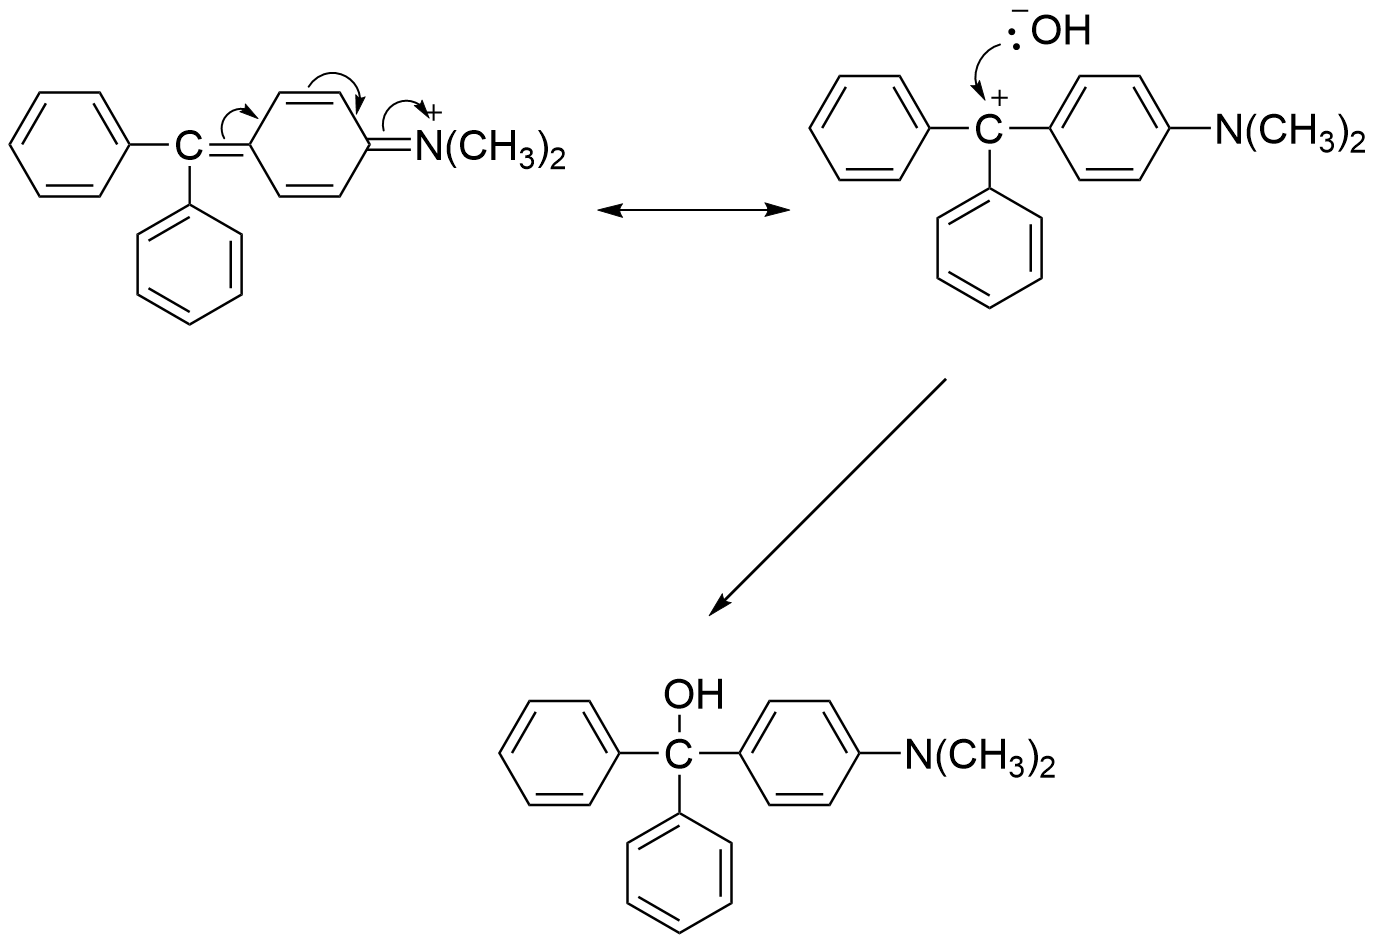
\includegraphics[width=\columnwidth]{malachite green.png}
    \caption{Reaction of malachite green with sodium hydroxide}
    \label{malachite green}
\end{figure}


In this experiment, the rate of this reaction were studied under different concentration of sodium hydroxide. Since malachite green had colour and the product was colourless, the reaction rate could be monitored by UV-Vis Spectroscopy. Based on the Beer-Lambert Law as shown in equation \ref{Beer-Lambert Law}, the absorbance of the solution was proportional to the concentration of malachite green. Therefore, the reaction rate could be calculated by measuring the absorbance of the solution at different time. 

\begin{equation}
    \label{Beer-Lambert Law}
    A = \epsilon l c
\end{equation}

Where A was the absorbance of the solution, $\epsilon$ was the molar absorptivity, l was the path length of the cuvette and c was the concentration of malachite green. When the hydroxyl ion was excess, the reaction rate followed pseudo-first order kinetics as shown in equation \ref{pseudo-first order kinetics}, where [MG]$_t$ represented the concentration of malachite green at any time, while [MG]$_0$ was when t=0. The pseudo-first rate constant was represented as k', which had the relationship with the second order rate constant k as shown in equation \ref{fk3}.

\begin{subequations}
    \label{pseudo-first order kinetics}
    \begin{gather}
        \frac{d[MG]_t}{dt} = -k ^{\prime} [MG]_0 \label{fk1}\\
        ln[MG]_t = -k ^{\prime} t + ln[MG]_0 \label{fk2}\\
        k ^{\prime} = k [OH^-] \label{fk3}
    \end{gather}
    % \label{pseudo-first order kinetics}
\end{subequations}

Because the concentration of malachite green was proportional to the absorbance of the solution, the absorbance of the solution could be used to calculate the reaction rate as shown in equation \ref{pseudo-first order kinetics2}. 

\begin{equation}
    \label{pseudo-first order kinetics2}
    ln \left | A \right |_t = -k ^{\prime} t + ln\left | A \right | _0
\end{equation}

Surfactants were amphiphilic molecules, which had both hydrophilic and hydrophobic parts. In this experiment, the surfactant was sodium dodecyl sulfate (SDS). The positive ions (Na$^+$) and the negative ions (DS$^-$) were able to move freely in the water, which made the solution conductive. 
The negatively charged part of SDS could form micelles in aqueous solution. The micelles were spherical, while the hydrophobic tails pointed inside and the hydrophilic heads pointed outside. The concentration when micelles could form spontaneously was called critical micelle concentration (CMC), which could be determined by measuring the conductivity of the solution.
% \hl{Surfactants or detergents are amphiphilic molecules whichundergo the self-assembly process known as micellizationthrough hydrophobic, electrostatic, or H-bonding interactions.}

% b\cite{intro}


% \hl{pectral and surface tension measurement studies onthe premicelle formation behavior of several carbocation dyeswith different anionic surfactants such as sodium dodecyl sulfate(SDS), sodium dodecyl benzenesulfonate (SDBS), and sodiumdodecyl sulfonate (SDSN) have been reported. The studies indicated the formation of dye-surfactant ion pairs (DSIP) at surfactant concentrations much below CMC. Such types of submicellar dye-surfactant interactions have also been found in our earlier studies involving the alkaline hydrolysis of crystal violet carbocation in the presence of anionic dye} 

% a\cite{intro16}


In this experiment, the rate of the reaction between malachite green and hydroxyl ions was studied. The pseudo-first order rate constant was calculated by measuring the absorbance of the solution using UV-Vis Spectroscopy. The second order rate constant was calculated. The CMC of SDS was determined by measuring the conductivity of the solution. The effect of SDS and the formation of micelle on the rate of the reaction between malachite green and hydroxyl ions was studied using UV-Vis Spectroscopy.





\section{Methodology}
\textbf{Part 1: Malachite green hydrolysis in water}\\
From the stock solution of NaOH (50 cm$^{3}$, 0.025 M), a series dilution was performed with deionised water to obtain solutions A-F with different concentration as shown in Table \ref{NaOH}. Malachite green (50 cm$^{3}$, 25 mg dm$^{-3}$) and NaOH solution A-F were warmed in 298 K water bath. The UV-1800 Shimadzu UV Spectrophotometer was used in this experiment with VICI DBS Single Cell Peltier System as temperature controller. Deionised water was used as Baseline measurement. When the temperature of the malachite green was stablised, its maximum absorbance was determined by measuring the absorbance of malachite green from 550 nm to 750 nm. The malachite green (1.5 cm$^3$) was mixed with NaOH solution A-F (1.5 cm$^3$) and the absorbance of each mixture was recorded at the maximum absorbance of malachite green for 5 minutes, and the temperature of each solution was recorded. Each measurement was repeated three times.\\

\begin{table}[h]
    \caption{Concentration of NaOH solutions A-F before mixing with malachite green [NaOH]$_i$, and after mixing with malachite green [NaOH]$_f$}
    \label{NaOH}
    \begin{tabular}{L{0.6in}C{1.2in}C{1.2in}}\toprule
        Solution &  [NaOH]$_0$ (M)   & [NaOH]$_f$ (M)\\\midrule
        A &   2.5 $\times 10^{-2}$    &   1.3 $\times 10^{-2}$ \\
        B & 1.3 $\times 10^{-2}$ &    6.3 $\times 10^{-3}$ \\
        C & 6.3 $\times 10^{-3}$& 3.1 $\times 10^{-3}$     \\
        D & 3.1 $\times 10^{-3}$ & 1.6 $\times 10^{-3}$      \\
        E & 1.6 $\times 10^{-3}$& 7.8 $\times 10^{-4}$   \\
        F & 7.8 $\times 10^{-4}$ & 3.9 $\times 10^{-4}$    \\\bottomrule
   \end{tabular}
\end{table}


\textbf{Part 2: Effect of Micelles on Reaction Kinetics}\\

Sodium dodcyl sulfate (SDS) (1\% w/v) was pipetted into 100 cm$^3$ volumetric flask, and diluted with deionised water to obtain solutions 1-6 with different concentration as shown in Table \ref{SDS}. During the dilution, deionised  water was carefully added into the solution along the glass wall to prevent bubble formation. 
Two potassium chloride solutions (30 cm$^3$, 0.001 mol dm$^{-3}$) and SDS solutions 1-8 was placed into the water bath (298 K) for 15 minutes. The conductivity of each SDS solution 1-8 was measured using the Jenway 4510 Conductivity Meter ($\kappa$ = 1.202) after calibrated with KCl solution. Each solution was measured for three times and the temperature of the solution was recorded each time. The conductivity another KCl solution was recorded to obtain the system error. 

\begin{table}[h]
    \caption{The volume of SDS and deionised water, and the concentration of SDS solutions 1-8}
    \label{SDS}
    \begin{tabular}{L{0.6in}C{0.8in}C{0.8in}C{0.8in}}\toprule
        Solution & V$_{SDS}$ (cm$^3$)& V$_{H_2O}$ (cm$^3$)& [SDS]   (\% w/v)\\\midrule
        1 & 1.00 & 99.00 & 0.01  \\
        2 & 5.00 & 95.00 &0.05  \\
        3 & 10.00&90.00&0.10  \\
        4 &20.00&80.00& 0.20     \\
        5 & 30.00&70.00&0.30 \\
        6 & 40.00&60.00&0.40 \\
        7 & 50.00&50.00&0.50 \\
        8 & 60.00&40.00&0.60 \\\bottomrule
   \end{tabular}
\end{table}

Sodium hydroxide (20 cm$^3$, 0.025 mol dm$^{-3}$) was mixed with different volume of SDS solution and deionised water to make solution A'-F' as shown in Table \ref{NaOHSDS}. The solution A'-F' and malachite green were placed into the water bath (298 K). The same measurement procedure was followed as in Part 1. \\

\begin{table}[h]
    \caption{The volume of SDS and deionised water, and the concentration of SDS solutions A'-F' before mixing with malachite green [SDS]$_i$, and after mixing with malachite green [SDS]$_f$}
    \label{NaOHSDS}
    \begin{tabular}{L{0.4in}C{0.7in}C{0.7in}C{0.6in}C{0.6in}}\toprule
        Solution & V$_{SDS}$ (cm$^3$)& V$_{H_2O}$ (cm$^3$)& [SDS]$_i$ (\%w/v)& [SDS]$_f$ (\%w/v)\\\midrule
        A' & 0 & 80 & 0 & 0\\
        B' & 10 & 70 &0.10 & 0.05\\
        C' & 20&60&0.20 & 0.10\\
        D' &40&40& 0.40  & 0.20\\
        E' & 60&20&0.60 & 0.30 \\
        F' & 80&0&0.80 & 0.40\\\bottomrule
   \end{tabular}
\end{table}



\section{Results}  


\textbf{Part 1: Malachite green hydrolysis in water}\\

The wavelength of the maximum absorbance of malachite green was obtained by measuring the absorbance of the malachite green from 550 nm to 750nm as shown in Figure \ref{maximumMG}. The maximum absorbance wavelength was 616 nm.

\begin{figure}[H]
    \centering
    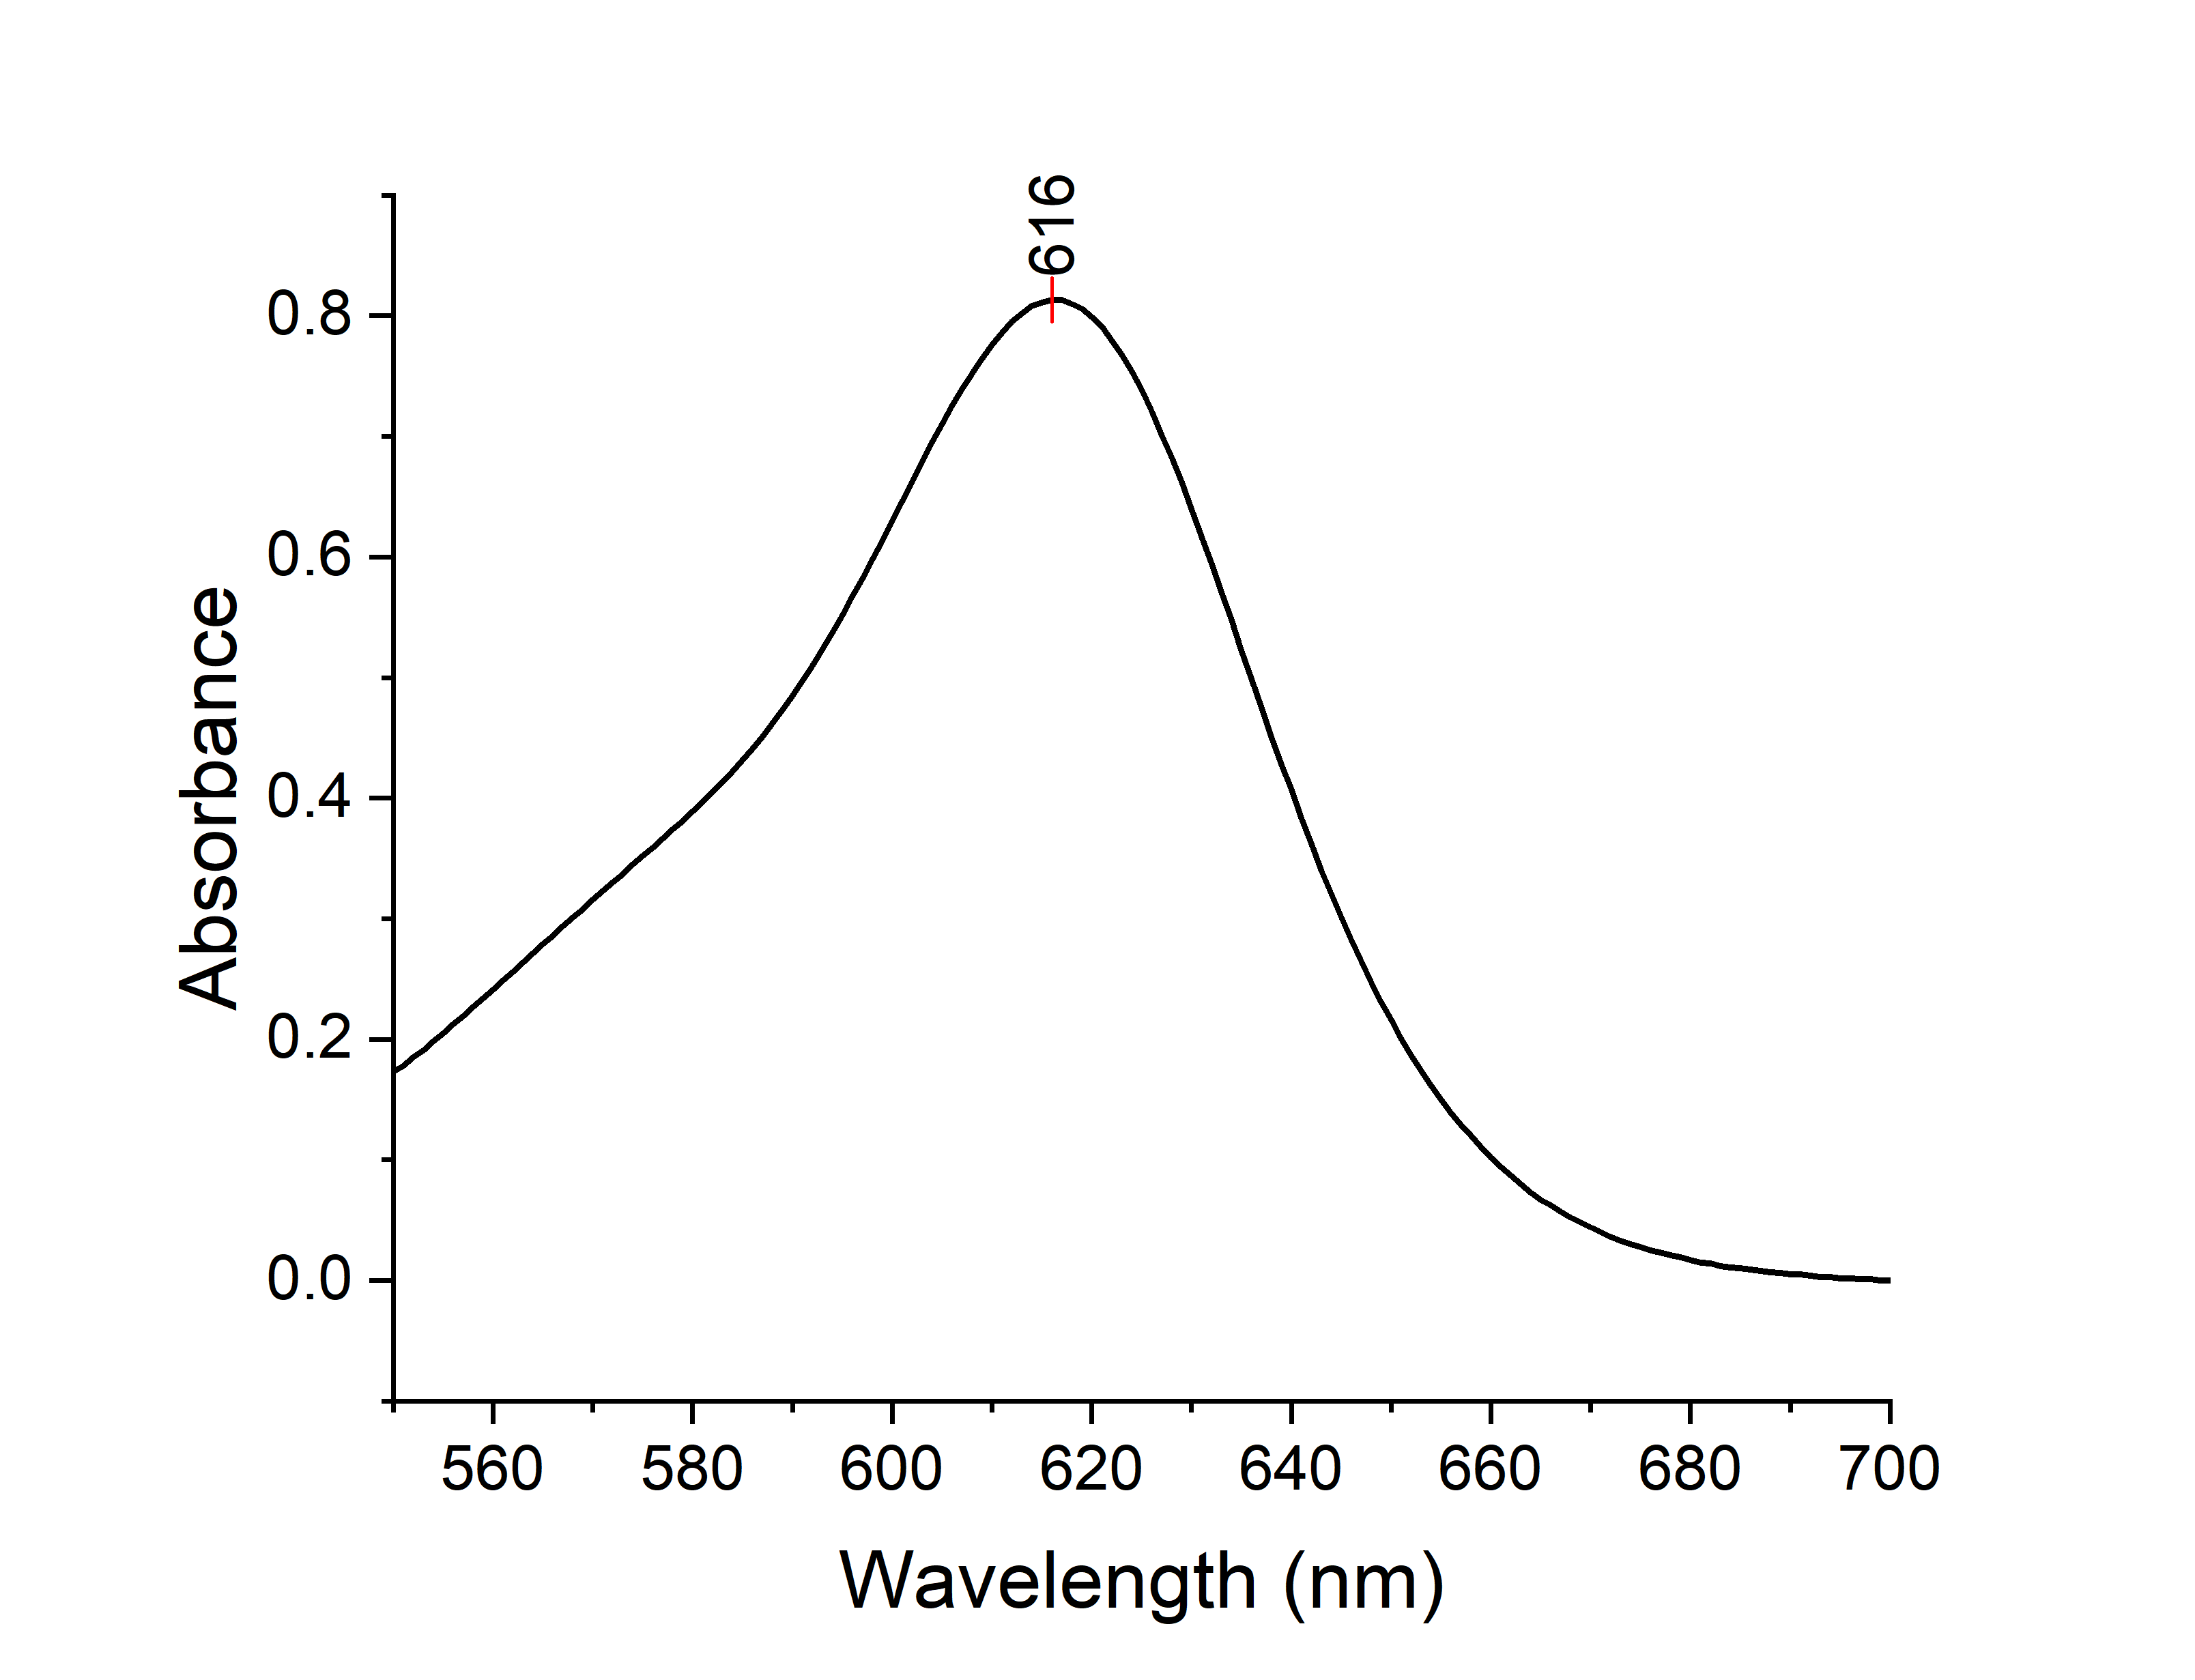
\includegraphics[width=\columnwidth]{max A of MG (1).png}
    \caption{The maximum absorbance of malachite green was obtained by measuring the absorbance of the malachite green from 550 nm to 750nm. The maximum absorbance wavelength was 616 nm.}
    \label{maximumMG}
\end{figure}


Malachite green was mixed with different concentration of sodium hydroxide solution A-F. The absorbance of the solution was decreased over time as malachite green was reacted to form a colourless product. The change of the absorbance (A) was recorded, and ln(A) was plotted against ln([OH$^-$]) as shown in Figure \ref{A}.

\begin{figure}[H]
    \centering
    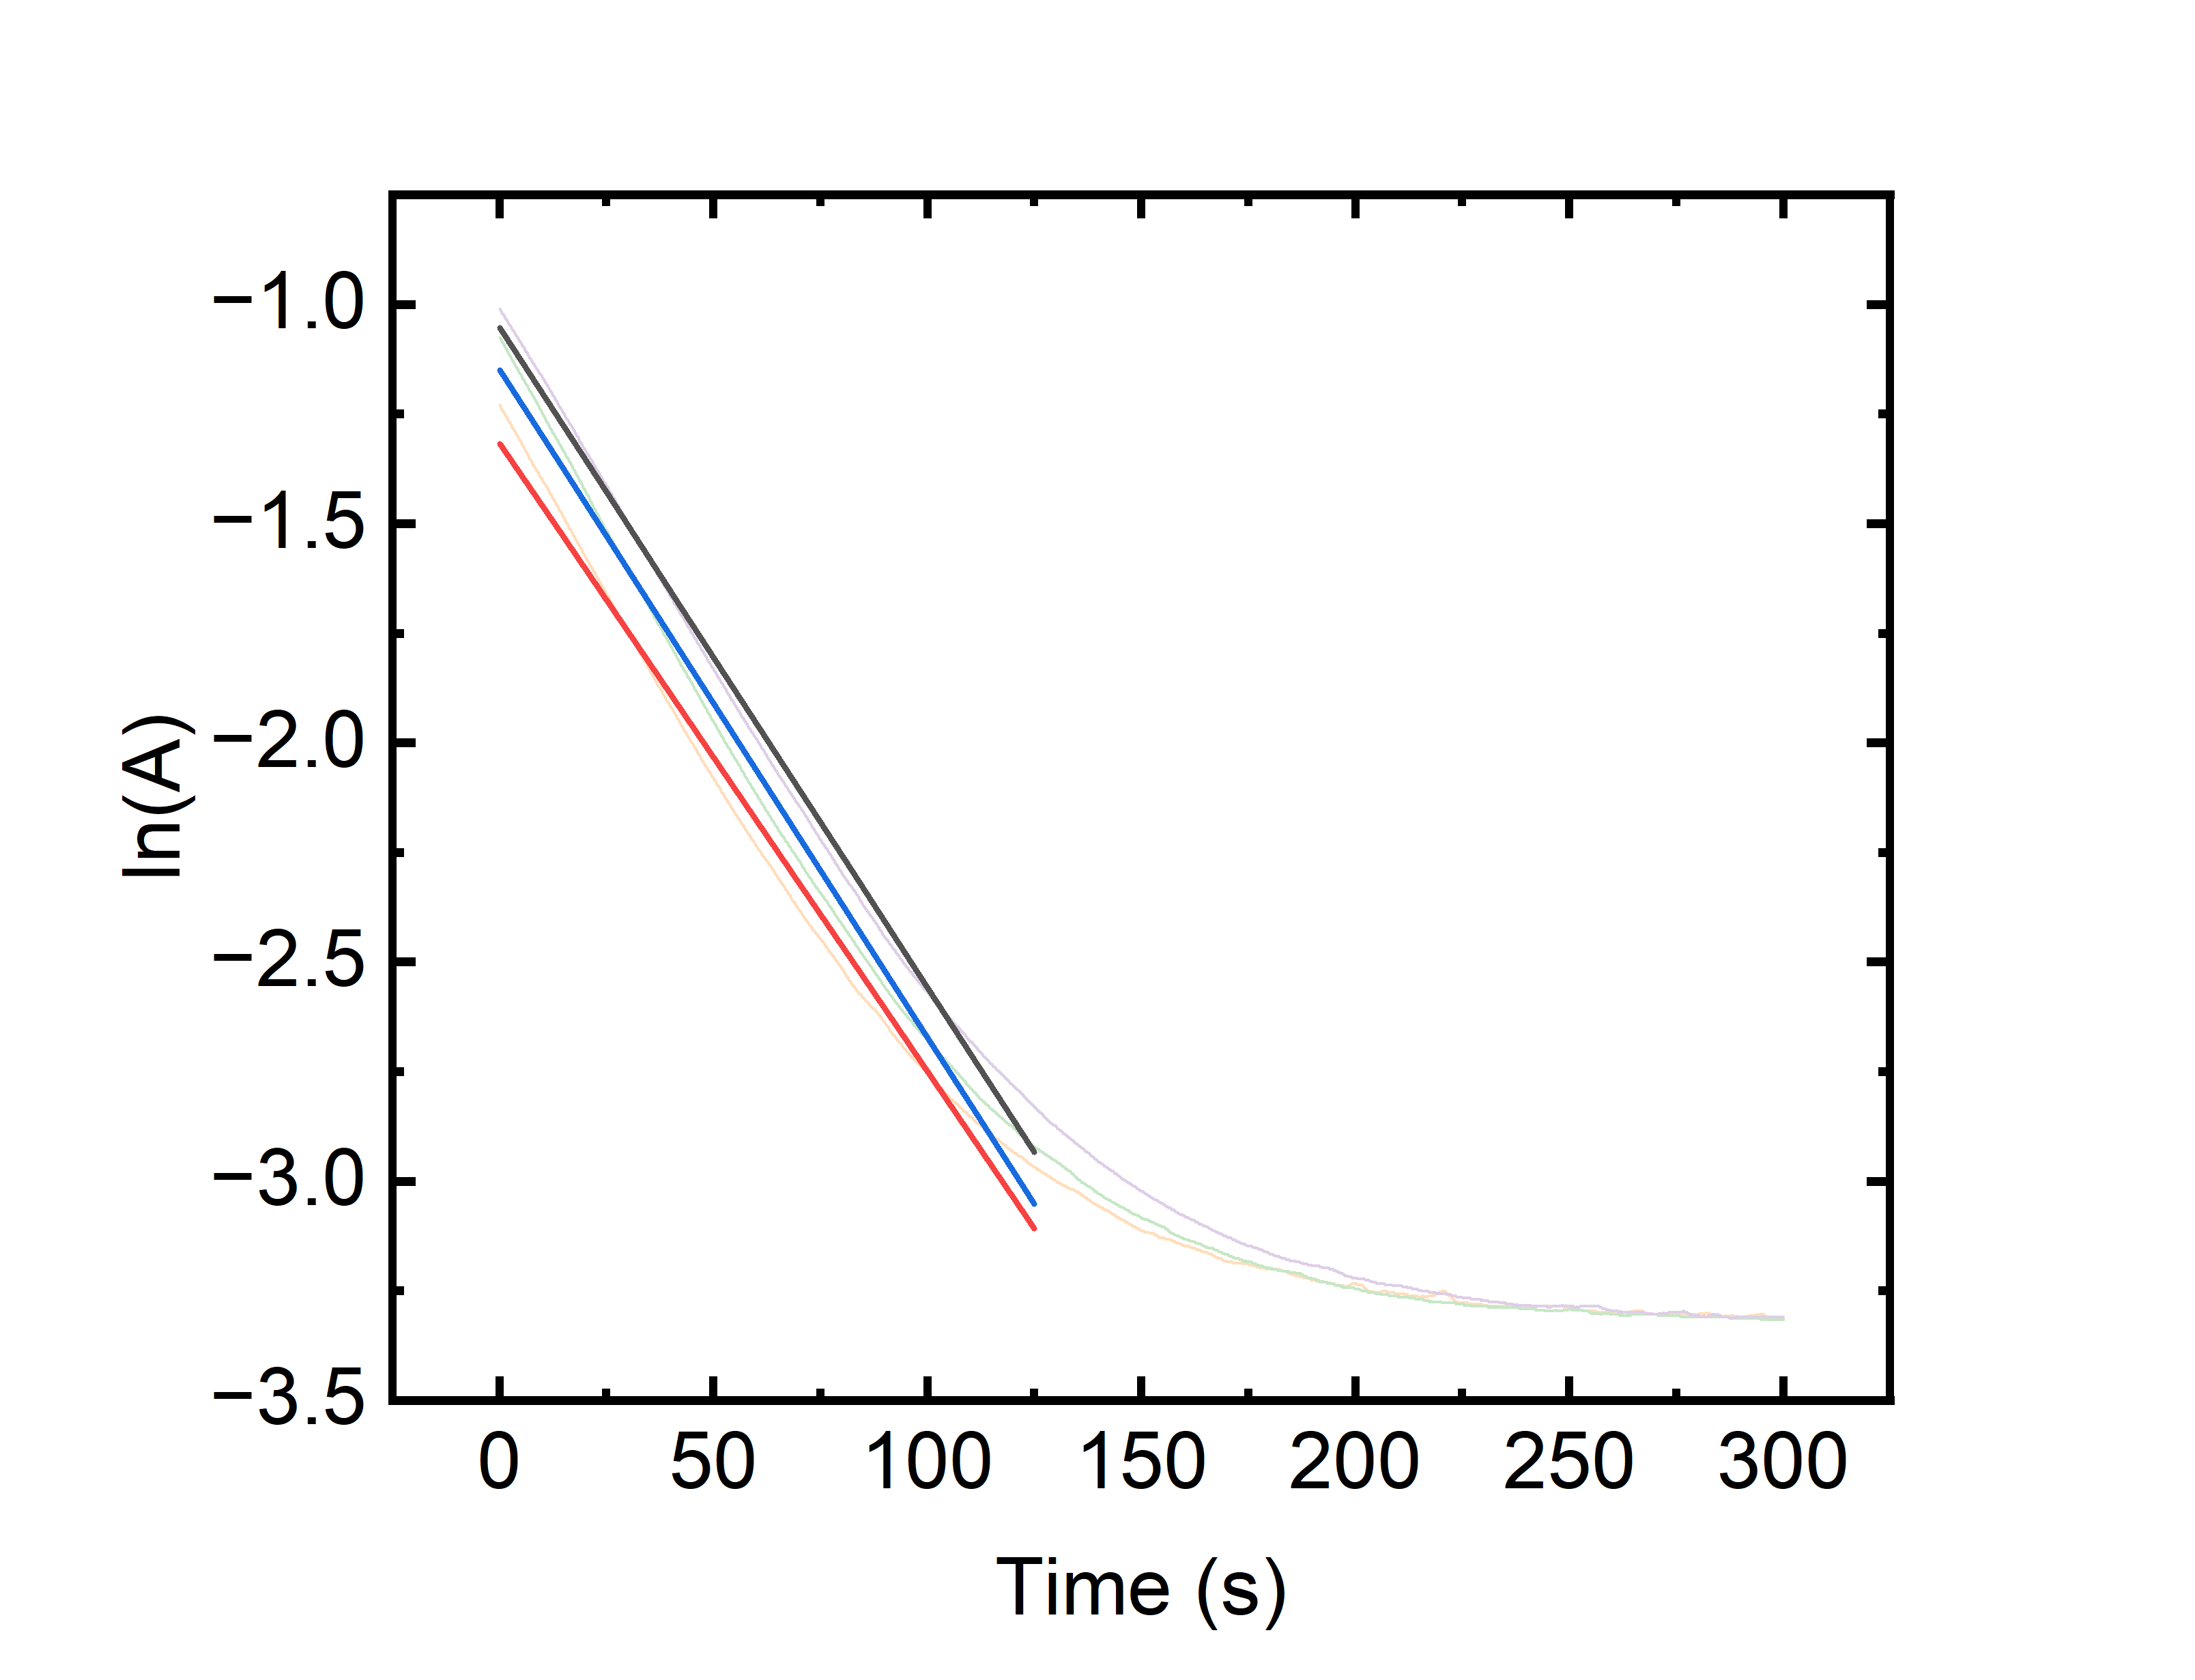
\includegraphics[width=\columnwidth]{part1A.png}
    \caption{The absorbance of the mixture of malachite green and solution A. The transparent line represented the original data, while the linear part of the graph was fitted using linear regression shown as the solid line. The slope of the black line was 1.51$\times 10^{-2}$ $\pm$ 4 $\times 10^{-5}$ with r$^2$ = 0.998, the slope of the blue line was 1.43$\times 10^{-2}$ with r$^2$ = 0.997, the slope of the red line was 1.52$\times 10^{-2}$ with r$^2$ = 0.997.}
    \label{A}
\end{figure}

The decrease of the absorbance become slower as the reagent decreased over time. The linear part of the graph was fitted using linear regression. The negative value of the slope was the pseudo-first order rate constant k' as shown in equation \ref{fk2}. The pseudo-first order rate constant k' was calculated for each solution A-F as shown in Table \ref{A-F}.


\begin{table}[h]
    \caption{The pseudo-first order rate constant k' of the reaction between malachite green and NaOH solution A-F, and each reaction was measured for three times}
    \label{A-F}
    \begin{tabular}{L{0.3in}C{0.9in}C{0.9in}C{0.9in}}\toprule
        Solution & 1  & 2 & 3  \\\midrule
        A' & 1.51$\times 10^{-2}$ $\pm$ 4 $\times 10^{-5}$ & 1.43$\times 10^{-2}$ $\pm$ 6 $\times 10^{-5}$  & 1.52$\times 10^{-2}$ $\pm$ 5 $\times 10^{-5}$   \\
        B' & 9.59$\times 10^{-3}$ $\pm$ 8 $\times 10^{-6}$ & 9.43 $\times 10^{-3}$ $\pm$ 8 $\times 10^{-6}$  & 9.18 $\times 10^{-3}$ $\pm$ 7 $\times 10^{-6}$   \\
        C' & 5.23 $\times 10^{-3}$ $\pm$ 3 $\times 10^{-6}$ & 5.06 $\times 10^{-3}$ $\pm$ 3 $\times 10^{-6}$  & 5.05 $\times 10^{-3}$ $\pm$ 3 $\times 10^{-6}$  \\
        D' & 2.91$\times 10^{-3}$ $\pm$ 9 $\times 10^{-7}$ & 2.78 $\times 10^{-3}$ $\pm$ 7 $\times 10^{-7}$  & 2.78 $\times 10^{-3}$ $\pm$ 9 $\times 10^{-7}$   \\
        E' & 5.77 $\times 10^{-4}$ $\pm$ 4 $\times 10^{-7}$ & 5.48 $\times 10^{-4}$ $\pm$ 3 $\times 10^{-7}$  & 5.18 $\times 10^{-4}$ $\pm$ 1 $\times 10^{-6}$   \\
        F' & 8.50 $\times 10^{-4}$ $\pm$ 3 $\times 10^{-7}$ & 8.60 $\times 10^{-4}$ $\pm$ 3 $\times 10^{-7}$  & 8.44 $\times 10^{-4}$ $\pm$ 3 $\times 10^{-7}$ \\\bottomrule
   \end{tabular}
\end{table}


The average value of the pseudo-first order rate constant k' was calculated as shown in Table \ref{A-F average}. The standard deviation of the pseudo-first order rate constant k' was calculated as shown in Table \ref{A-F average}.\\[1\baselineskip]

\begin{table}[h]
    \caption{The average pseudo-first order rate constant k' of the reaction between malachite green and NaOH solution A-F, the standard deviation was calculated, and the temperature of each solution was recorded}
    \label{A-F average}
    \begin{tabular}{L{0.4in}C{1in}C{1in}C{0.6in}}\toprule
        Solution & Average k$^\prime$ (s$^{-1}$)& Standard deviation & Temperature ($^\circ$C)\\\midrule
        A' & 1.48$\times 10^{-2}$ & 4.82 $\times 10^{-4}$  & 24\\
        B' & 9.40$\times 10^{-3}$ & 2.07 $\times 10^{-4}$  &24 \\
        C' & 5.11$\times 10^{-3}$ & 1.01 $\times 10^{-4}$ &24\\
        D' & 2.82$\times 10^{-3}$ & 7.05 $\times 10^{-5}$ &24 \\
        E' & 5.63$\times 10^{-4}$ & 2.04 $\times 10^{-5}$ &24\\
        F' & 8.51$\times 10^{-4}$ & 7.72 $\times 10^{-6}$ &24\\\bottomrule
   \end{tabular}
\end{table}

The second order rate constant k could be obtained as shown in equation \ref{fk3}. The average pesudo-first order rate constant k' was plotted against the concentration of OH$^-$ as shown in Figure \ref{k}. The slope of the graph was the second order rate constant k.

\begin{figure}[H]
    \centering
    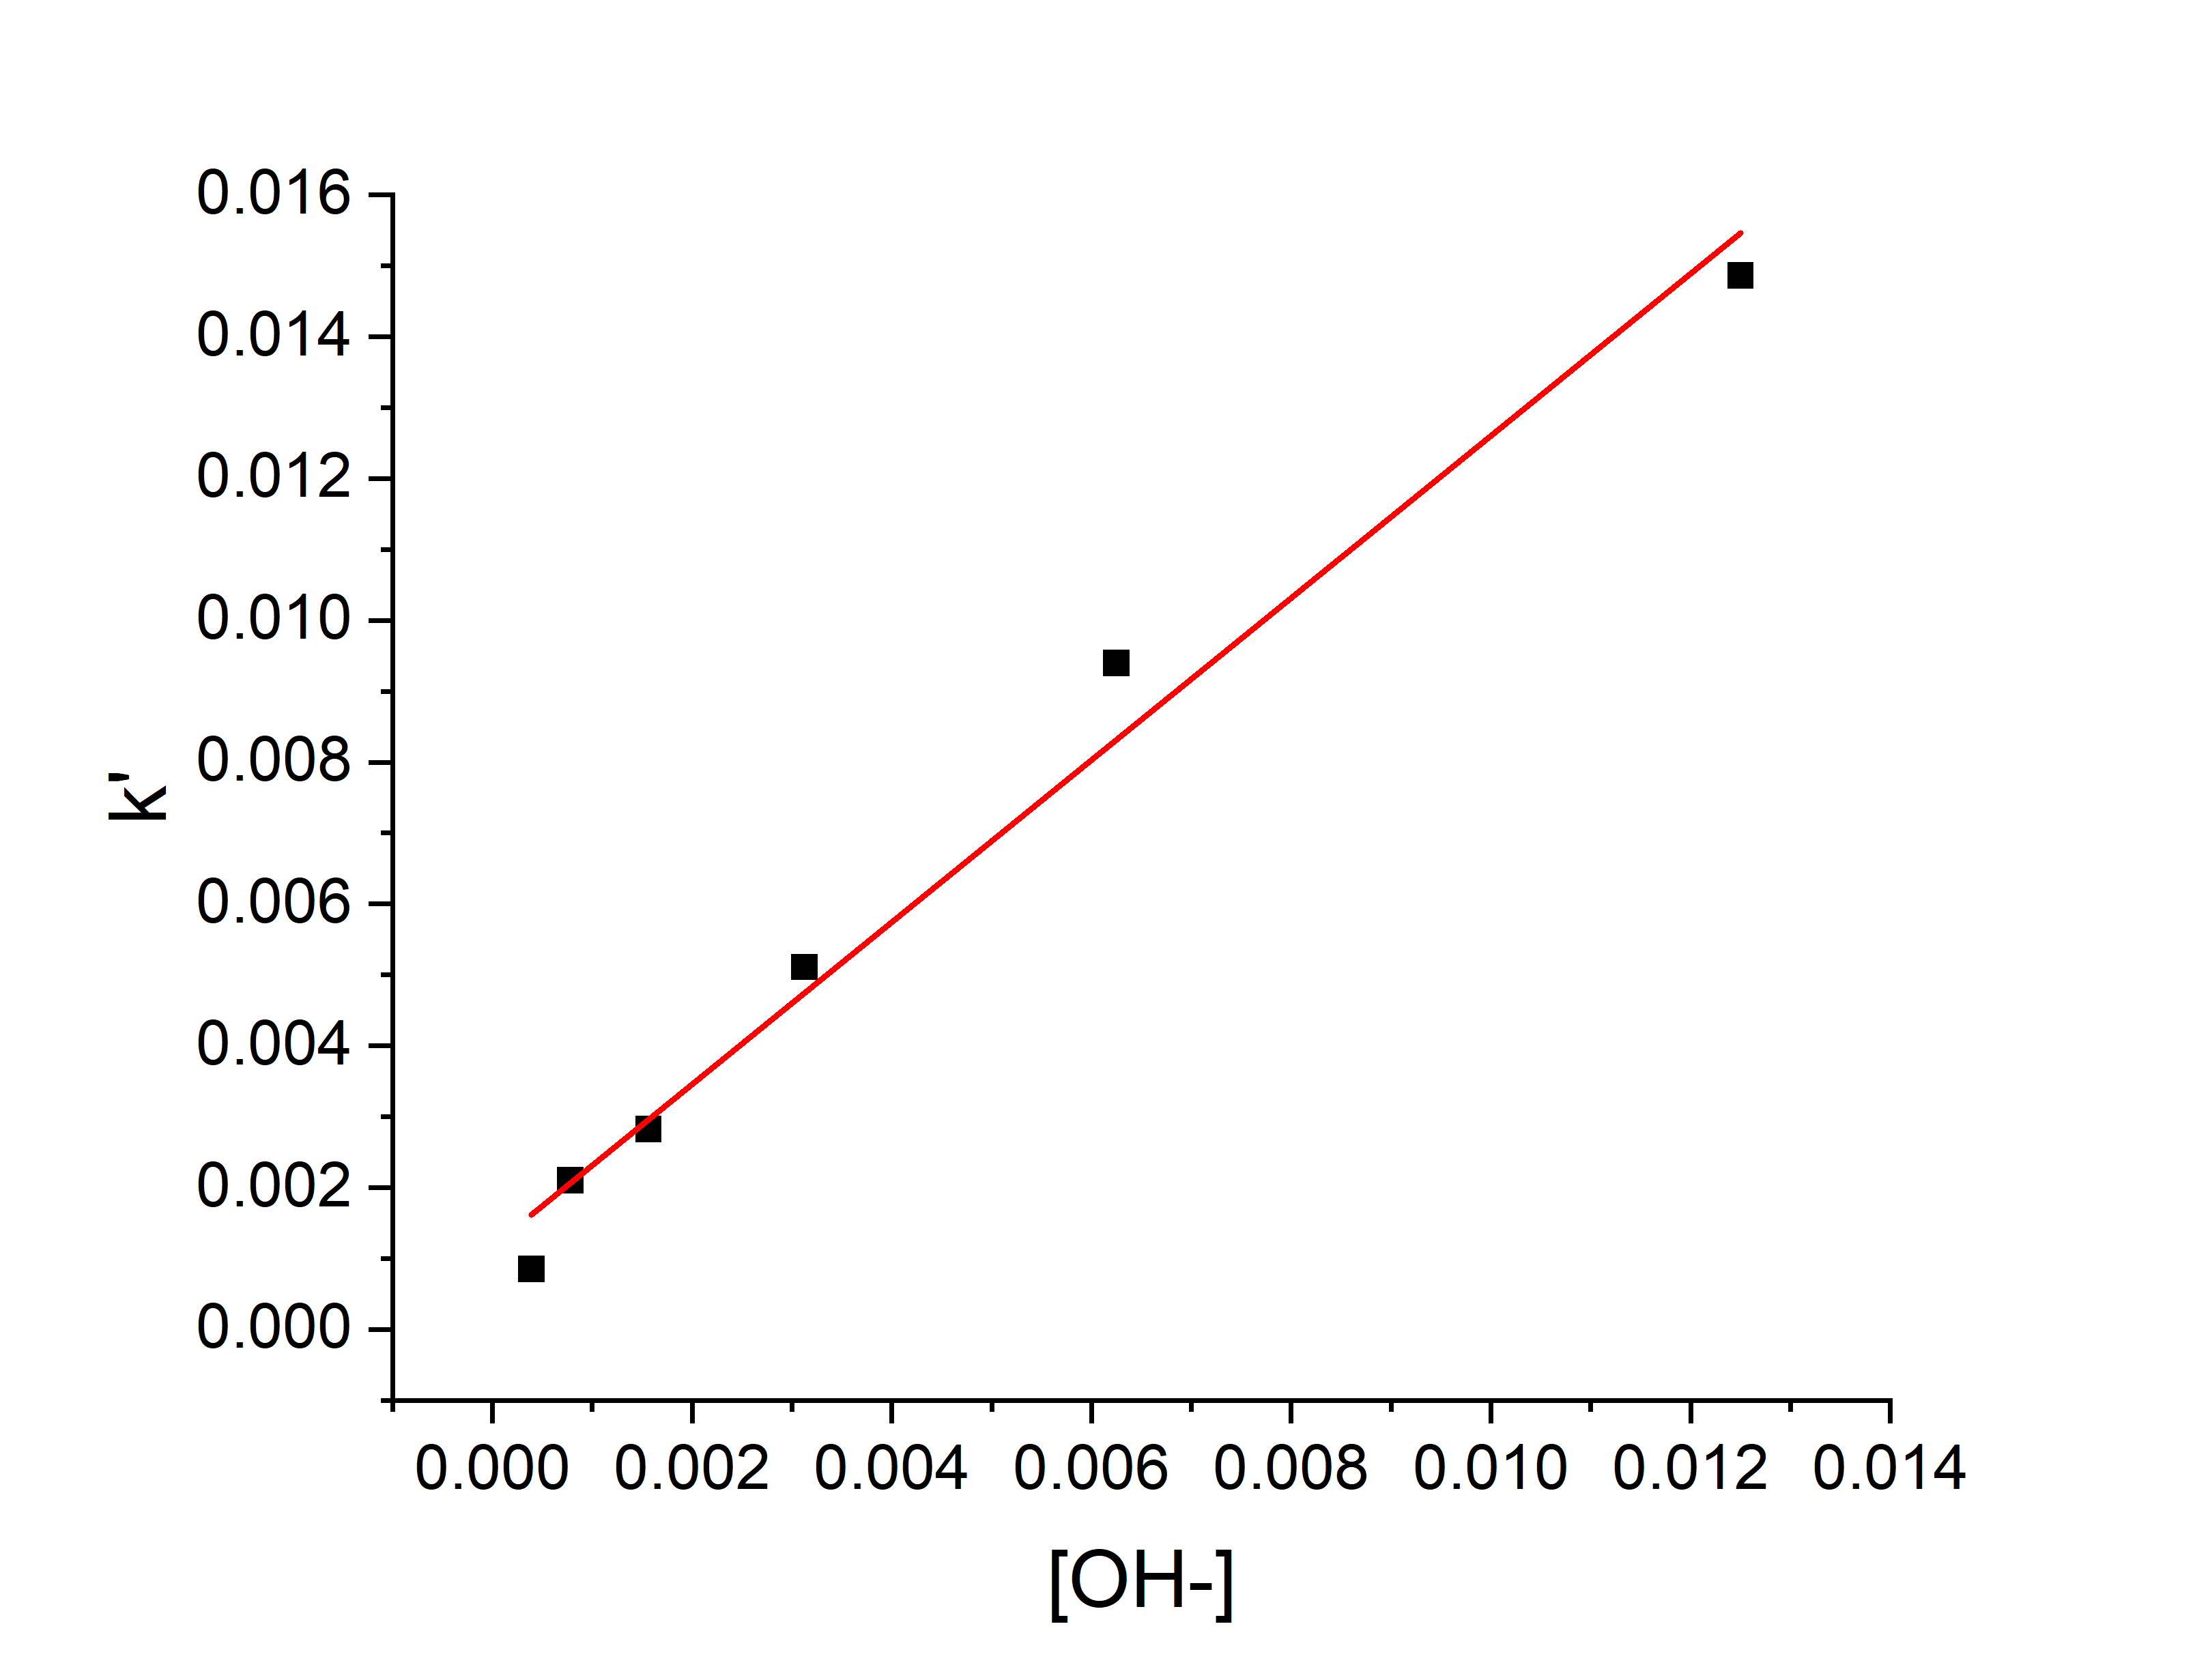
\includegraphics[width=\columnwidth]{part1 k.png}
    \caption{The pseudo-first order rate constant k' was plotted against the concentration of OH$^-$,the slope of the graph was 1.143 $\pm$ 0.07 with r$^2$ = 0.992.}
    \label{k}
\end{figure}




% \textbf{Part 2: Effect of Micelles on Reaction Kinetics}\\
% \begin{table}[h]
%     \caption{Rate of the reaction between malachite green and solution A'-F', each reaction was repeated three times, and the average rate was calculated}
%     \label{NaOHSDS}
%     \begin{tabular}{L{0.3in}C{0.6in}C{0.6in}C{0.6in}C{0.6in}C{0.3in}}\toprule
%         Solution & 1  & 2 & 3 & average & error \\\midrule
%         A' & -4.47$\times 10^{-3}$ $\pm$ 3 $\times 10^{-6}$ & -4.57$\times 10^{-3}$ $\pm$ 3 $\times 10^{-6}$  & -4.64$\times 10^{-3}$ $\pm$ 2 $\times 10^{-6}$  & -4.47$\times 10^{-3}$ $\pm$ 3 $\times 10^{-6}$ & \\
%         B' & 1.50 & 1.00 &0.00 & & \\
%         C' & 1.50&2.00&0.00 & &\\
%         D' &1.50&3.00& 0.00  &  & \\
%         E' & 1.50&4.00&0.00 & & \\
%         F' & 1.50&5.00&0.00 & & \\\bottomrule
%    \end{tabular}
% \end{table}

\textbf{Part 2: Effect of Micelles on Reaction Kinetics}\\

The conductivity of SDS solution different concentration 1-8 was measured as shown in Figure \ref{conductivity}. The conductivity of the SDS solution increased with the increase of the concentration of SDS. However, there was a turning point where the increase of the conductivity slowed down, this was the CMC of SDS as shown in Figure \ref{conductivity}. 

\begin{figure}[H]
    \centering
    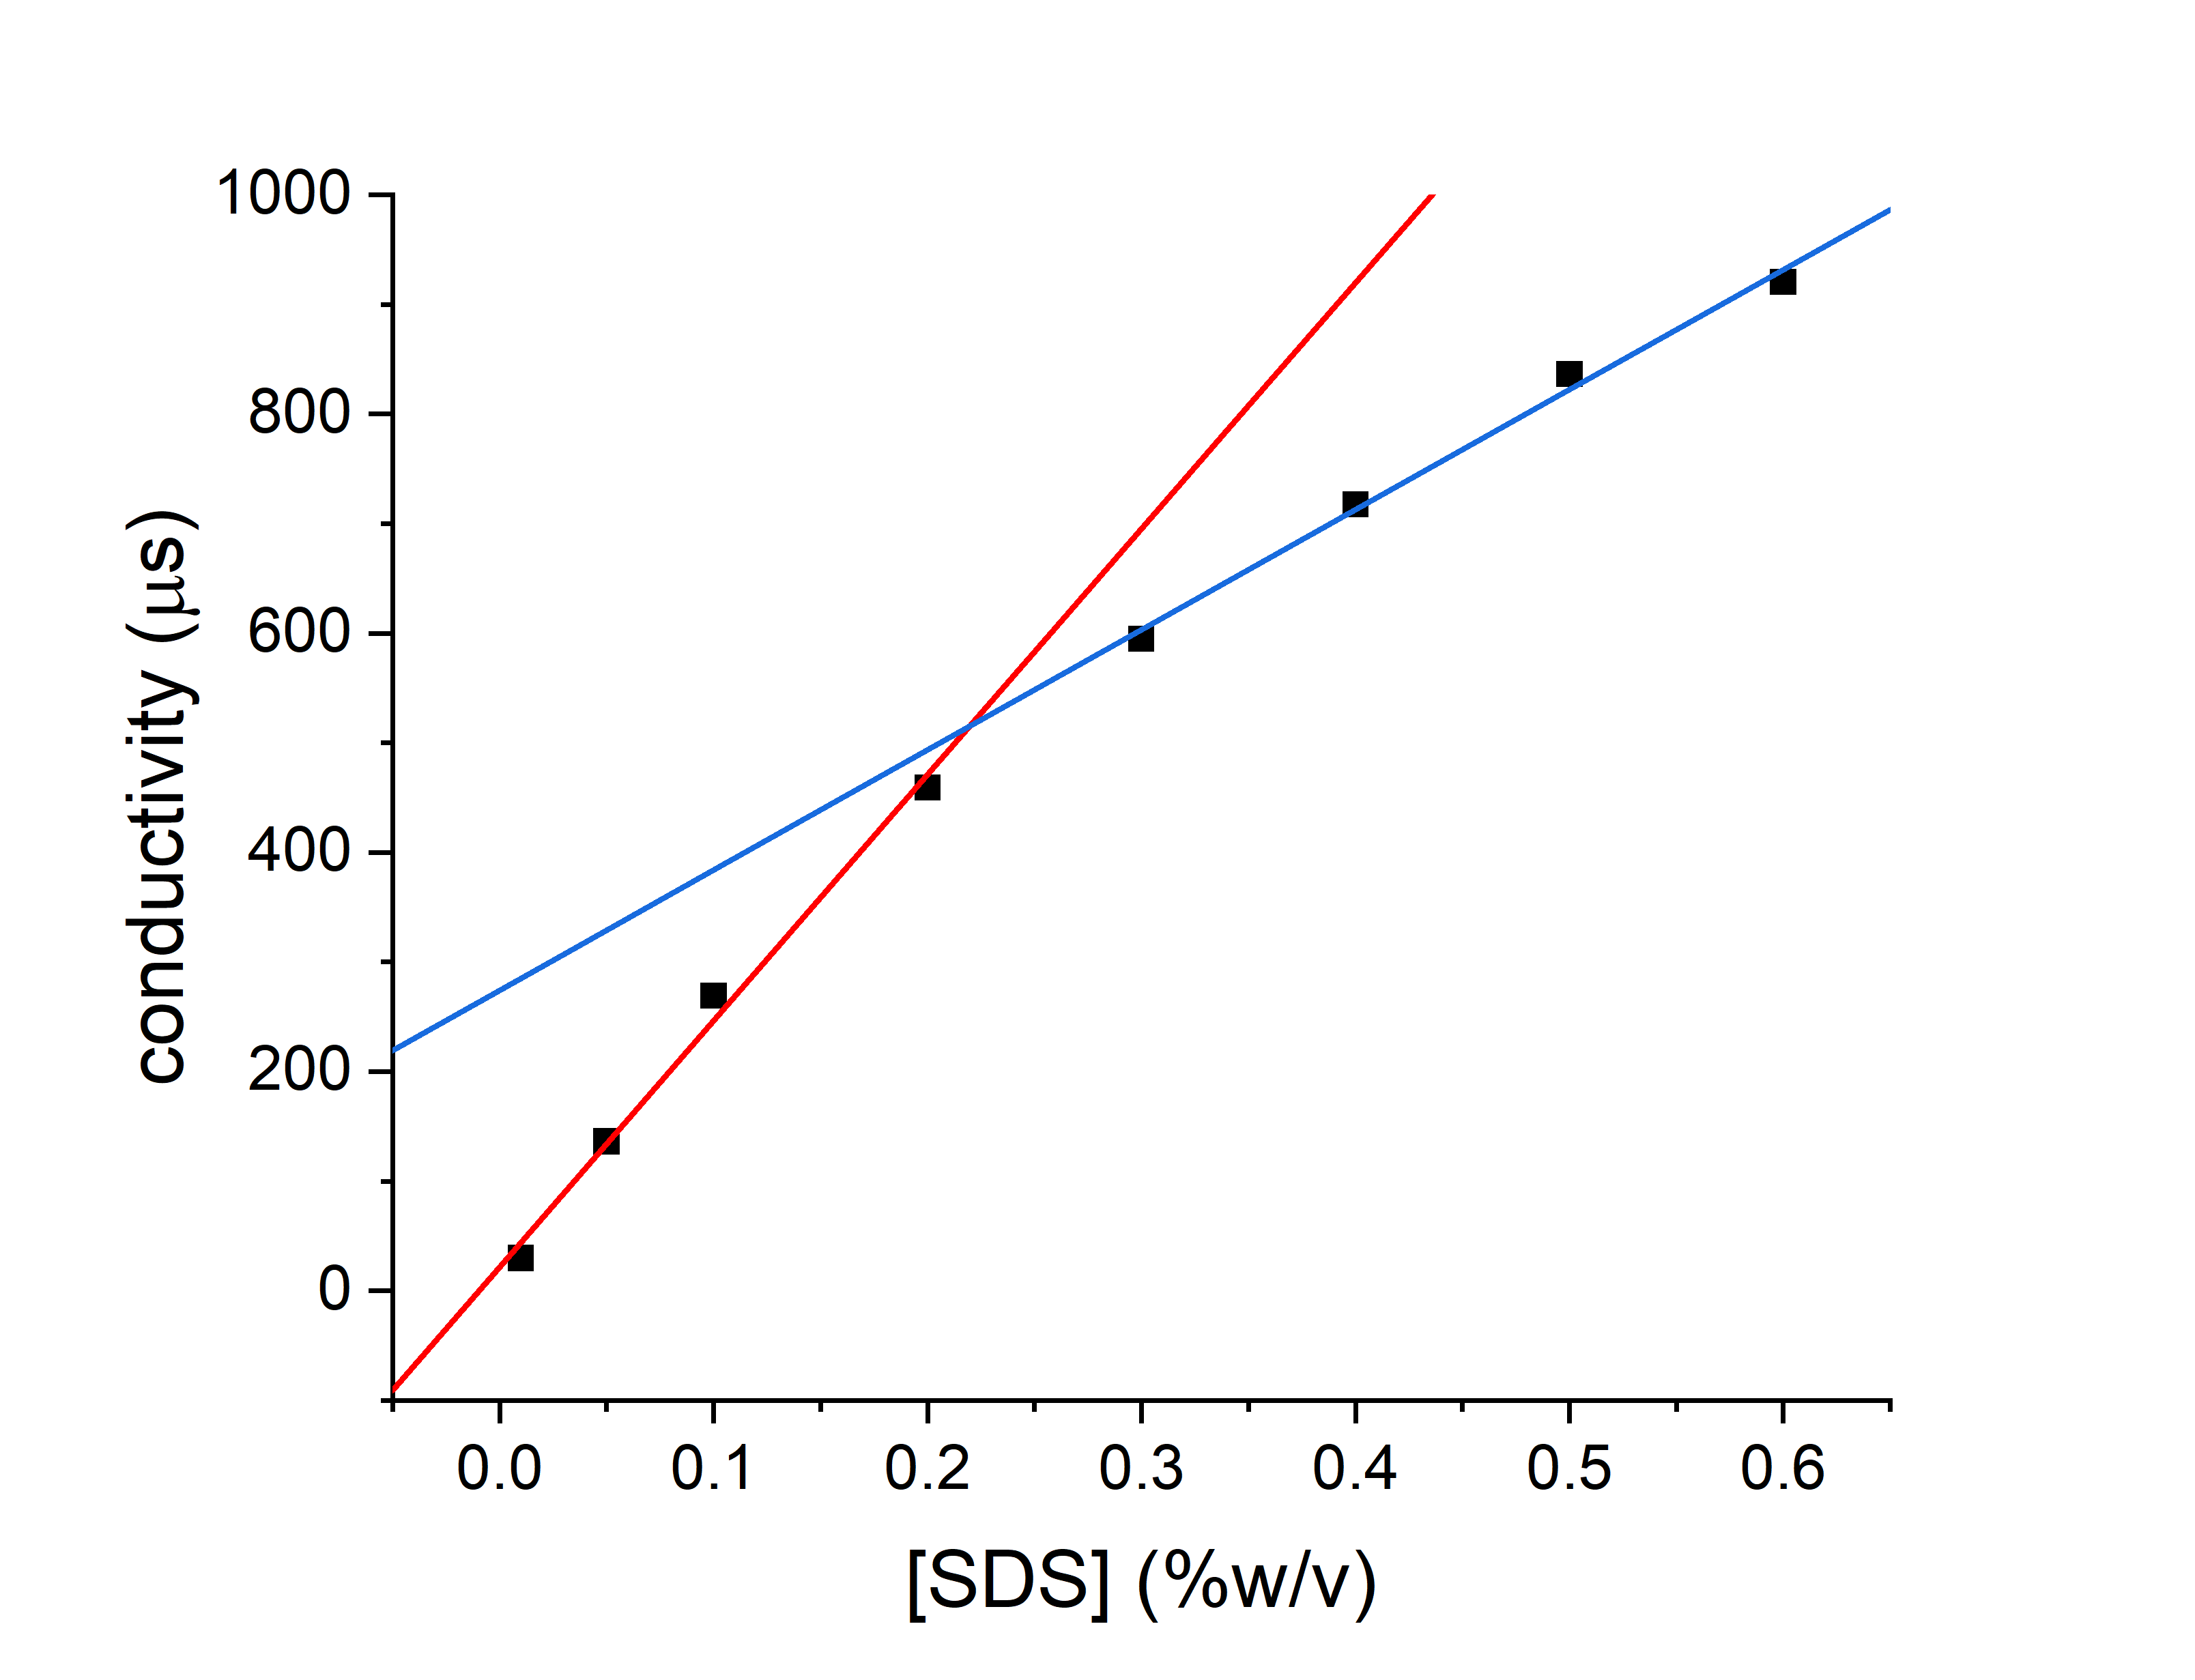
\includegraphics[width=\columnwidth]{part2 CMC.png}
    \caption{The conductivity of SDS solution different concentration 1-8. The red line was the linear regression before the CMC, while the blue line was the linear regression after the CMC. The linear function of the red line was $y= (2245 \pm 100) x + 21.55 \pm 10$ with r$^2$ = 0.997, the linear function of the blue line was $y= (1096 \pm 60) x 274.2 \pm 30$ with r$^2$ = 0.996.}
    \label{conductivity}
\end{figure}

The CMC of SDS could be obtained by solving the linear function of the red line and the blue line as shown, which was 0.219 $\pm$ 0.004\%w/v, which equaled to 7.59 $\times 10^{-3}$ $\pm$ 1 $\times 10^{-5}$ mol L$^{-1}$.

The effect of SDS and the formation of micelle on the rate of the reaction between malachite green and hydroxyl ions was studied. Since the rate of the reaction could be calculated as shown in equation \ref{fk1} and the concentration of the malachite green was proportional to the absorbance of the solution as shown in equation \ref{Beer-Lambert Law}, the rate of the reaction could be represented as the decrease of the absorbance over time. Therefore, the absorbance of the solution was plotted against time, and the negative value of the slope could represent the rate of the reaction as shown in Table \ref{RateSDS}.


\begin{table}[h]
    \caption{Rate of the reaction between malachite green and solution A'-F', each reaction was repeated three times}
    \label{RateSDS}
    \begin{tabular}{L{0.3in}C{0.9in}C{0.9in}C{0.9in}}\toprule
        Solution & 1  & 2 & 3  \\\midrule
        A' & 1.38$\times 10^{-3}$ $\pm$ 2 $\times 10^{-5}$ & 1.40 $\times 10^{-3}$ $\pm$ 4 $\times 10^{-5}$  & 1.37 $\times 10^{-3}$ $\pm$ 4 $\times 10^{-5}$   \\
        B' & 8.51 $\times 10^{-5}$ $\pm$ 9 $\times 10^{-8}$ & 8.59 $\times 10^{-5}$ $\pm$ 9 $\times 10^{-8}$  & 8.38 $\times 10^{-5}$ $\pm$ 1.14 $\times 10^{-7}$   \\
        C' & 8.44 $\times 10^{-5}$ $\pm$ 5 $\times 10^{-8}$ & 8.42 $\times 10^{-5}$ $\pm$ 4 $\times 10^{-7}$  & 7.85 $\times 10^{-5}$ $\pm$ 3 $\times 10^{-7}$   \\
        D' & 8.58 $\times 10^{-5}$ $\pm$ 5 $\times 10^{-8}$ & 8.51 $\times 10^{-5}$ $\pm$ 5 $\times 10^{-8}$  & 7.63 $\times 10^{-5}$ $\pm$ 3 $\times 10^{-8}$  \\
        E' & 6.10 $\times 10^{-5}$ $\pm$ 8 $\times 10^{-8}$ & 6.10 $\times 10^{-5}$ $\pm$ 8 $\times 10^{-8}$  & 6.00 $\times 10^{-5}$ $\pm$ 7 $\times 10^{-8}$  \\
        F' & 5.75 $\times 10^{-5}$ $\pm$ 9 $\times 10^{-8}$ & 5.93 $\times 10^{-5}$ $\pm$ 1 $\times 10^{-7}$  & 5.94 $\times 10^{-5}$ $\pm$ 1 $\times 10^{-7}$   \\\bottomrule
   \end{tabular}
\end{table}


The average value of the slope and the standard deviation were calculated as shown in Table \ref{NaOHSDS average}.

% \begin{table}[]
%     \begin{tabular}{llllll}
%     0.001383333 & 8.49181E-05 & 8.23712E-05 & 8.23943E-05 & 5.86932E-05 & 6.06695E-05 \\
%     1.52753E-05 & 1.0803E-06  & 3.36474E-06 & 5.26472E-06 & 1.01498E-06 & 5.66092E-07
%     \end{tabular}
% \end{table}

\begin{table}[h]
    \caption{Average rate of the reaction between malachite green and solution A'-F' and the standard deviation was calculated}
    \label{NaOHSDS average}
    \begin{tabular}{L{0.4in}C{1.3in}C{1.3in}}\toprule
        Solution & Average  rate & Standard deviation \\\midrule
        A' & 1.38 $\times 10^{-3}$ & 1.53 $\times 10^{-5}$   \\
        B' & 8.49 $\times 10^{-5}$ & 1.08 $\times 10^{-6}$   \\
        C' & 8.24 $\times 10^{-5}$ & 3.36 $\times 10^{-6}$ \\
        D' & 8.24 $\times 10^{-5}$ & 5.26 $\times 10^{-6}$ \\
        E' & 5.87 $\times 10^{-5}$ & 1.01 $\times 10^{-6}$ \\
        F' & 6.06 $\times 10^{-5}$ & 5.66 $\times 10^{-7}$ \\\bottomrule
    \end{tabular}
\end{table}






The average rate of the reaction was plotted against the concentration of SDS as shown in Figure \ref{MGCMC}. The rate decreased dramatically when SDS was added to the solution, and the rate decreased slowly when SDS concentration was increased. The first three data was fitted using linear regression, and the last three data was fitted using linear regression. The cross point of the two linear regression was identified as the CMC of SDS as shown in Figure \ref{MGCMC}, which was 0.08295 $\pm$ 0.03\%w/v, which equaled 2.876 $\times 10^{-3}$ $\pm$ 1 $\times 10^{-5}$ mol L$^{-1}$.

\begin{figure}[H]
    \centering
    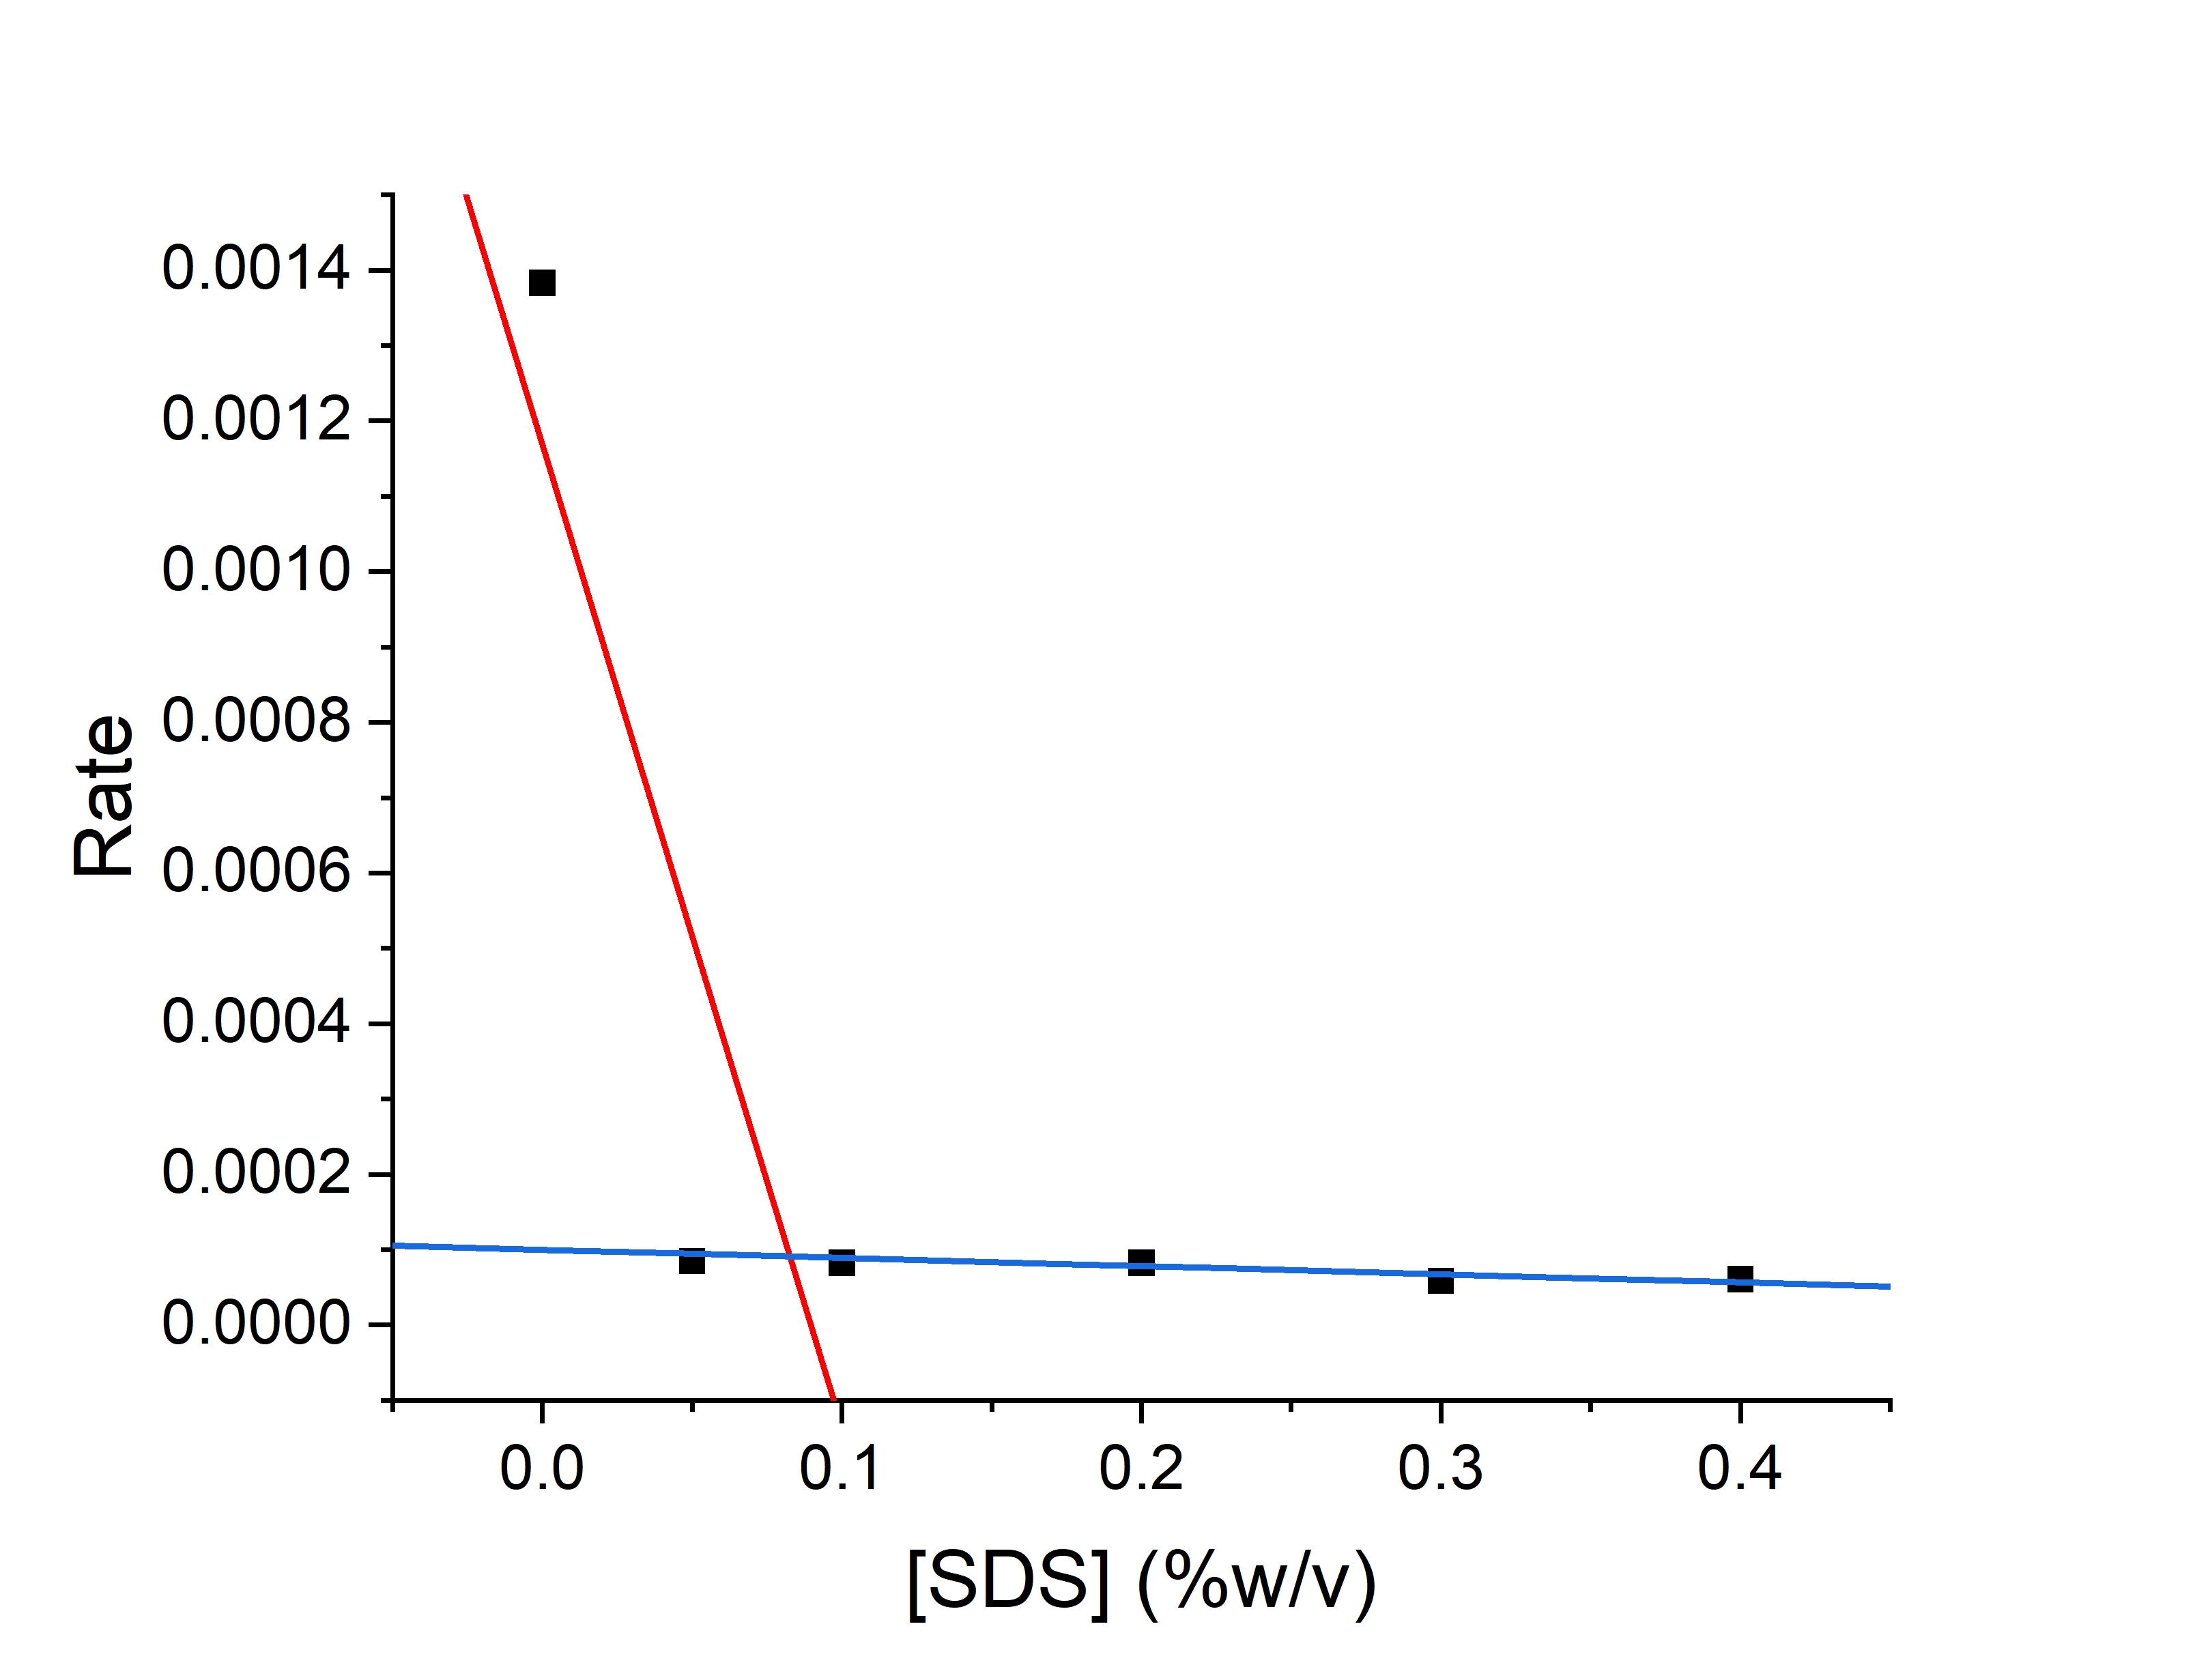
\includegraphics[width=\columnwidth]{CMC2 (1).png}
    \captionof{figure}{The average rate of the reaction was plotted against the concentration of SDS. The first three data was fitted using linear regression shown as the red line, which had linear function as $y = (-0.01301 \pm 0.007)x + 0.00117 \pm 5 \times 10^{-4}$  with r$^2$ = 0.867. The last three data was fitted using linear regression shown as the blue line, which had linear function as $y = ( -1.086 \times 10^{-4} \pm 7 \times 10^{-5})x + 9.98 \times 10^{-5}\pm 2 \times 10^{-5}$  with r$^2$ = 0.826. The cross point of the two linear regression was identified as the CMC of SDS, which was 0.08295 $\pm$ 0.03\%w/v.}
    \label{MGCMC}
\end{figure}


\section{Discussion}

% \hl{short summary}

The maximum absorbance of malachite green was observed at 616 nm as shown in Figure \ref{maximumMG}. This wavelength was chosen to measure the absorbance of the solution to maximize the sensitivity of the UV-Vis spectrum. 

The absorbance of the solution for each mixture of malachite green and NaOH solution A-F was measured for three times. The standard deviation  of the pseudo first order kinetic constant k was calculated as shown in Table \ref{A-F average}. The standard deviation of the pseudo first order kinetic constant k was small, which indicated that the experimental data was reliable and reproduced. The largest standard deviation was the reaction between malachite green and solution E because the concentration of the sodium hydroxide was very low and the reaction would be very slow, which indicated that small change of the volume of sodium hydroxide during the measurement would cause large change of the concentration of hydroxyl ions, leading to the change of the rate. 

The second rate constant was obtained based on the pseudo first order kinetic constant k, which was 1.143 $\pm$ 0.07 $L$ $mol^{-1}s{-1}$. The literature value of the second order kinetic constant of the reaction between malachite green and hydroxyl ions was 1.428 $\pm$ 0.025 $L$ $mol^{-1}s{-1}$.\cite{intro} The percent error was calculated as shown in equation \ref{error}, which was 20\%. The large percent error might due to the difference of the temperature of the solution. The temperature of the solution was in this experiment was lower than the literature value, which might lead to a lower rate of the reaction, resulting a smaller value of second order kinetic constant.
\begin{equation}
    \label{error}
    \% error = \frac{1.428-1.143}{1.428} \times 100\%
\end{equation}

Sodium dodecyl sulfate (SDS) had a positively charged part (Na$^+$) and a negatively charged part (C$_12$H$_25$SO$_4^-$). The negatively charged part was amphiphilic, meaning that it had a hydrophilic part and a hydrophobic part. In aqueous solution, it could form a micelle, where the hydrophilic part pointing outside, and the hydrophobic part pointing inside. The formation of micelle was driven by thermodynamics, which was mainly due to the increase of the entropy of H$_2$O.

The effect of SDS on the rate of the reaction between malachite green and hydroxyl ions was studied. The CMC of SDS was determined by measuring the conductivity of the solution, which was 7.59 $\times 10^{-3}$ $\pm$ 1 $\times 10^{-5}$ mol L$^{-1}$. The literature value of the CMC of SDS was 7.26 $\times 10^{-3}$ mol L$^{-1}$.\cite{intro} The percentage error between the experimental data and the literature value was 4.5\%. The percentage error was very small, which indicated the CMC value measured in this experiment was accurate. 

The reaction rate was measured under different concentration of SDS. When the SDS was added to the solution, the reaction rate dropped dramatically. This was because that SDS had a negatively charged part (C$_{12}$H$_25$SO$_4^-$), which could interact with the positively charged malachite green forming a dye-surfactant ion-pair based on the Oslo-Simonson Model.\cite{21} Since SDS had a long bulky tail, it might cause steric hindrance, which would prevent the attack of hydroxyl ions to the malachite green.

Instead of the one-to-one association described in the Oslo-Simonson Model, Piszkiewicz Cooperativity Model suggested that n number of negatively charged part of SDS would interact with one malachite green to form a premicelle complex (S$^-_n$---MG$^+$).\cite{22}The formation of premicelle complex provide a greater steric hindrance, which caused the reaction rate to decrease largely. 

A more recent study proved that as the concentration of SDS increase, ion-pair micelles would form as shown in Figure \ref{ion-pair micelle}.\cite{intro16} When the concentration of SDS reached the CMC, normal micelle would form, and the negatively charged surface would interact with the micelle. The micelles had negative charge on the surface, which would repel the negatively charged hydroxyl ions, preventing the reaction between malachite green and hydroxyl ions. Therefore, the reaction rate decreased a lot as SDS added to it. 

\begin{figure}[H]
    \centering
    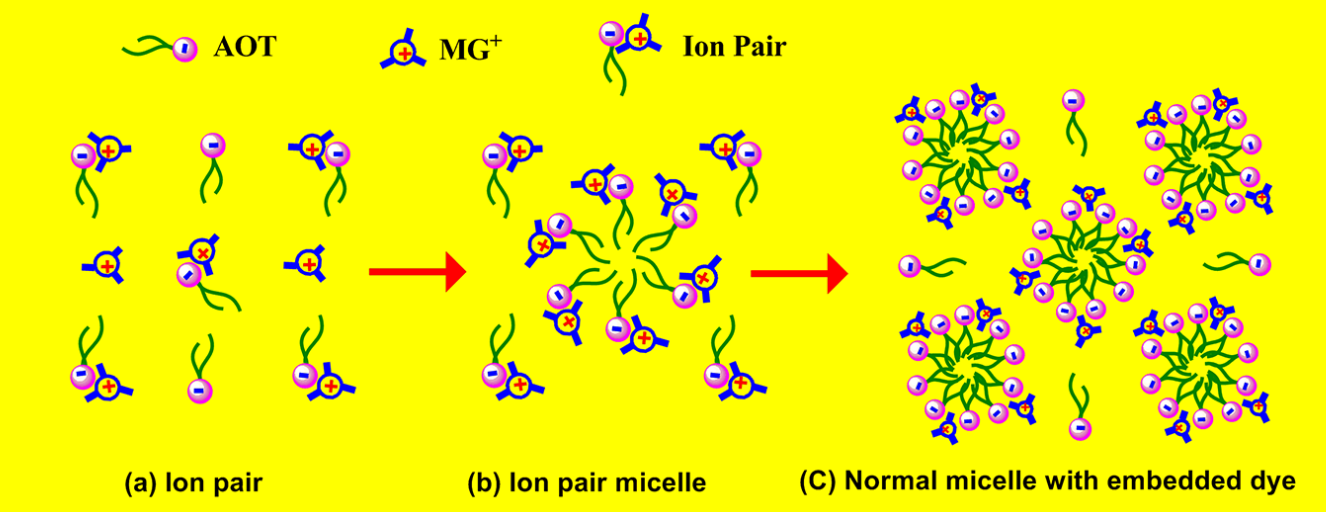
\includegraphics[width=\columnwidth]{ion-pair micelle.png}
    \caption{The formation of ion-pair micelle. The negatively charged part of SDS interacted with the positively charged malachite green to form ion-pair micelle.\cite{intro}}
    \label{ion-pair micelle}
\end{figure}

The critical micelle concentration was determined based on the change of the rate as change of the concentration of SDS, which was 2.876 $\times 10^{-3}$ $\pm$ 1 $\times 10^{-5}$ mol L$^{-1}$. This value was much lower than the CMC in deionised water. The CMC of SDS in NaOH was compare to the literature value, which was 3.27 $\times 10^{-3}$ mol L$^{-1}$.\cite{intro} The percentage error was calculated as 12\%. The difference between the CMC of SDS in deionised water and NaOH was due to the presence of more free ions in the solution as NaOH was a strong base and would fully dissociate in water. The large percentage error might due to that the concentration of NaOH was low, and the effect of SDS would be large even with a small amount. Therefore, the rate of the reaction was nearly zero when SDS was introduced into the solution. 

One possible experimental error in this experiment might be that the temperature of the solution was not stable, which might affect the rate of the reaction. This could be improved by increasing the time for waiting the temperature to be stable. Another possible experimental error might be that the concentration of the solution was not accurate due to the bubble forming when adding SDS, which might lead to different rate. This could be improved by slowly adding water into the SDS solution along the glass wall to prevent bubble forming. The rate of the reaction with the presence of SDS solution might be inaccurate because the concentration of SDS was very low, and the reaction rate was nearly zero. This error was most likely effect the data  because the change of the rate was too small when increasing the concentration of SDS, resulting difficulty in determining the CMC of SDS solution. This could be improved by increasing the concentration of NaOH in the solution. 


The rate of the reaction between malachite green and sodium hydroxide was monitored by UV-Vis Spectrophotometer in this experiment. The pseudo first order kinetic constant was determined under different concentration of NaOH. The second order kinetic constant was determined as 1.143 $\pm$ 0.07 $L$ $mol^{-1}s{-1}$, with 20\% error as compared to the literature value. The effect of SDS on the rate of the reaction between malachite green and hydroxyl ions was studied. The critical micelle concentration (CMC) of SDS in deionised water was determined as 7.59 $\times 10^{-3}$ $\pm$ 1 $\times 10^{-5}$ mol L$^{-1}$ based on the change of conductivity. The rate of the reaction was measured under different concentration of SDS. The critical micelle concentration was determined based on the rate change as 2.876 $\times 10^{-3}$ $\pm$ 1 $\times 10^{-5}$ mol L$^{-1}$. The rate of reaction was decreased dramatically when SDS was added to the solution. The effect of micelle was relatively small as the reaction rate was almost zero after adding a small amount of SDS. Errors in this experiment might include the unstable temperature of the solution, the inaccurate concentration of the solution due to bubble, and the small change of rate of the reaction with the presence of SDS solution. 


%\textbf{part2: Effect of Micelles on Reaction Kinetics}

% \hl{With further increase in surfactant concentration, these ion-pairs tend to aggregate to form ion-pair micelles\cite{intro16}(shown inFigure8) at a certain surfactant concentration, known as ion-pair CMC(CMCIP)(Figure 7). These ion-pair micelles, sometimes calledpremicelles\cite{25}}

% \hl{At this stage the ion-pairs dissociate, and the free cationicdye species are solubilized by the normal micelles.\cite{intro}}

% \hl{n. The CMCIPvalues for SDS and AOT arefound to be 5.95 $\times$ 10$^{-4}$ and 0.98 $\times$ 10$^{-4}$mol L$^{-1}$, respectively,which are much lower than their normal CMC values, viz., 7.26 $\times$ 10$^{-3}$and 1.68 $\times$ 10$^{-3}$ mol L$^{-1}$ \cite{intro}}


% \hl{ In the ion-pair micelles,only a small number of ion-pair units aggregate owing to thesteric hindrance of the electrostatically bound bulky head groupsresulting in a small decrease in free energy ($\Delta$G). When thesurfactant concentration is large, much larger number of puresurfactant monomers aggregate to form stable normal micellesresulting in a large decrease in free energy (due to hydrophobicinteraction). Possibly this latter large decrease in $\Delta$G more than compensates the small increase in $\Delta$G due to the breaking of theion pair micelle\cite{intro}}


\section{Investigation Question}
%this is a citation \cite{Example}

The concentration of the malachite green could be measured using UV-Vis Spectroscopy. The absorbance of the solution was proportional to the concentration of the malachite green as shown in equation \ref{Beer-Lambert Law}.

Hypothesis: The concentration of malachite green could be measured using UV-Vis Spectroscopy by measuring the absorbance of the solution.

Experiment: The absorbance of malachite green with different concentration from 1 mg dm$^{-3}$ to 100 mg dm$^{-3}$ was measured using UV-Vis Spectroscopy. The absorbance of the solution was measured at the maximum absorbance wavelength of malachite green, which was 616 nm. The absorbance of the solution was plotted against the concentration of malachite green. The linear function could be determined. The absorbance of the sample malachite green would be recorded. The concentration of sample malachite green could be calculated based on the absorbance of the solution using the linear function of the graph. 

The temperature of each malachite green solution should be the same in order to reduced the effect of temperature on the absorbance of the solution. The impurities in the malachite green sample might also affect the result. This could be improved by measuring the baseline with the sample solution that did not contain malachite green.



\bibliography{ref} %This command generates your bibliography. PLEASE MAKE SURE TO CHANGE THE NAME IN THESE CURLY BRACKETS TO WHATEVER YOUR .BIB FILE IS CALLED!!
\bibliographystyle{rsc} %setting for the RSC's .bst (style) file -- do NOT change this, unless you wish to define a new citation style

\end{document}


%Best of luck with your report! 

%Last SideNote: If you have any questions ask them during the lab session, you should have plenty of time and opportunity to go over everything. If you need more help once your sessions are over and you can't figure something out yourself, you can contact me at angie.matusova@ed.ac.uk. Please, don't hesitate to get in touch if you're struggling with something (though, please make sure you've exhausted all the other options before contacting me; i.e. you've reviewed all the material available on Learn and/or tried looking up your query online).